\chapter[ARQUITETURA PARA PROCESSAMENTO DE DADOS]{ARQUITETURA PARA PROCESSAMENTO DE DADOS}
\label{chapter:architecture}

A \textbf{Arquitetura Kappa} é o padrão de projeto escolhido para servir de
base para a camada de processamento de dados do InterSCity. A Arquitetura
Lambda não justifica a maior complexidade no contexto atual da plataforma, de
modo que essa escolha facilita a manutenibilidade e adoção da arquitetura pelo
time atual do InterSCity. A Arquitetura Kappa permitirá a análise em tempo-real
sem que ocorra perda de informações relevantes, o que é importante no contexto de
cidades inteligentes, ao passo em que permite a análise de dados históricos,
desde que estes tenham sido pré-processados. Esta decisão então trás a
necessidade de escolha de uma tecnologia de processamento \textit{streaming},
e de um \textit{broker} adequado.

O \textbf{Apache Spark} é a tecnologia de \textit{streaming} escolhida,
principalmente por dispor nativamente de biblioteca de clusterização e
aprendizagem de máquina. Esta ferramenta ainda facilita, caso necessário, a
troca para a Arquitetura Lambda, por dispor de processamento \textit{batch}.
O \textbf{Apache Kafka} é o \textit{broker} escolhido, sendo esta uma escolha
menos óbvia que a anterior. Embora o RabbitMQ já seja utilizado pelo
InterSCity, e tenha vantagens em certos aspectos em relação ao Kafka, não
dispor de uma interface nativa que o conecte ao Spark resultou nessa decisão.
Outro fator é o gerenciamento nativo de \textit{log} por parte do
Kafka, que ajuda na implantação da Arquitetura Kappa. O Kafka, contudo, só
será utilizado na camada de processamentos, não forçando mudanças no
ecossistema de microsserviços do InterSCity. A Figura \ref{fig:stack} ilustra
a pilha de tecnologias que deve compor a Arquitetura Kappa no InterSCity.

\begin{figure}
  \centering
    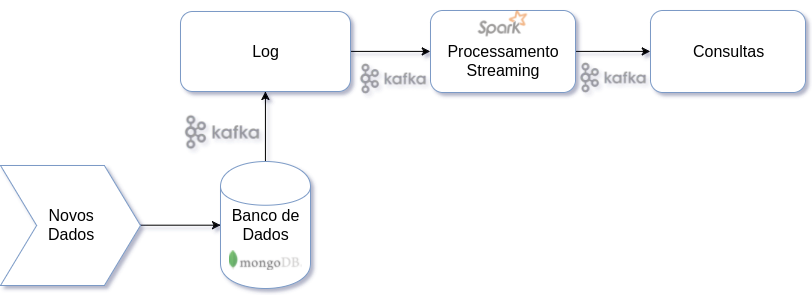
\includegraphics[scale=0.5]{figuras/kappa_tools.png}
  \caption{Pilha de tecnologias utilizadas - Apache Kafka, Apache Spark e MongoDB.}
  \label{fig:stack}
\end{figure}


\section{IMPLEMENTAÇÃO}

A implementação da arquitetura foi dividida em três etapas: (i)
configuração do ambiente, contemplando as ferramentas escolhidas; (ii)
ligações entre os diferentes projetos, tornando possível a publicação de
mensagens no Kafka e sendo possível seu processamento no Spark; e (iii)
disponibilização de \textit{hooks} que possam ser extendidos futuramente,
possibilitando a criação de um \textit{pipeline de dados}. A implementação
trouxe para o InterSCity um novo Data Processor, e um componente chamado
\textbf{Shock}, responsável por abstrair as comunicações entre as diferentes
ferramentas, e por trazer a extensibilidade mencionada na terceira etapa da
implementação. Pseudo-algorítmos presentes no apêndice \ref{appendix:impl}
ilustram o uso das ferramentas escolhidas na implementação da Arquitetura
Lambda.

A configuração do ambiente, assim como seguido pelo time do InterSCity, foi
guiada pelo uso de conteinêres do Docker. Uma configuração do Spark
que já havia sido desenvolvida pelo time do InterSCity foi reutilizada,
precisando de poucas mudanças. Um conteinêr com o Kafka foi então configurado e
ligado aos conteinêres do Spark e do microsserviço Resource Adaptor, finalizando
assim esta etapa da implementação.

A ligação entre os projetos teve início com uma adaptação no microsserviço
Resource Adaptor, que, com a mudança, passa a publicar no tópico
\textit{new\_data}, no Kafka, a atualização de novos dados. Esta
adaptação não trouxe mudanças significativas no InterSCity, não afetando o
fluxo usual da plataforma. Foi desenvolvido então o Shock\footnote{O Shock e o
novo Data Processor estão no mesmo repositório: \url{https://gitlab.com/DGuedes/data-processor}
}, responsável por receber mensagens em tópicos específicos do Kafka, e
passá-los ao Spark Streaming. O Shock roda \textit{micro-batches} do Spark em
intervalos de tempos definidos previamente, e em cada um destes processamentos,
\textit{hooks} extensíveis são executados. Caso queira-se anexar mais uma
tarefa no \textit{pipeline de dados}, basta então registrá-la no Shock e
fornecer uma prioridade, que define se uma tarefa deve ser executada antes ou
depois no Shock.
